\section{Approaching high densities: supercooled liquids and glasses}
\label{sec:glass}

%% \subsection{Mean-field picture}
%% The infinite dimensional limit $d \to \infty$.

%% \subsection{Random first-order transition theory}
%% Perturbation from mean-field in $1/d$.

%% \subsection{Alternative pictures in physical dimensions}
%% For $d \le 3$
%% \subsubsection{Frustration-limited domain theory}
%% \subsubsection{Dynamical theories}

%% \subsection{Old intro stuff}

%% It is widely reported that glass is actually liquid, and as evidence of this the thickness of old windows at the bottom is pointed to.
%% This is actually a matter of some dispute, but contains a grain of truth.
%% Pre-modern methods of creating window glass involved spinning molten glass on magma to flatten it out.
%% Centrifugal forces caused the glass to be thicker on the outer disc, so panes of glass would always be heavier in one direction%
%% \marginfootnote{And personally, if I were setting an uneven pane of glass I would place the thicker and heavier part at the bottom.}.

%% To a soft matter physicist glass is a broader term, referring to a wide class of materials while the window glass of common parlance is referred to by its chemical name \emph{silicate}.
%% This class of materials share many features of being disordered etc \cite{?} although in some sense they are connected by what they do \emph{not} do: which is flow on human timescales.
%% When I refer to `glass' I will be using it in this broad technical sense of a state of matter.
%% Some examples besides silicate:
%% \begin{itemize}
%% \item Most of the ice in the universe exists in an amorphous state in comets \cite{?}
%% \item Ceramics
%% \item Plastics: amorphous polymers
%% \end{itemize}
%% Of more abstract nature which could be called glassy though they are not materials
%% \begin{itemize}
%% \item Gels: super glasses, liquid like bit plus a network/backbone which has glassy dynamics
%% \item Neural networks
%% \item Non-deterministic polynomial time (NP) problems
%% \end{itemize}
%% We will not be directly addressing the latter type of more abstract problems which could be considered glasses, although they are arguably related due to a similar underlying disorder.
%% We will be focusing on only the most rudimentary of glassy phenomenology: the dynamical arrest of liquids at high densities/low temperatures when crystallisation is avoided.
%% Especially as it manifests in hard spheres, which as discussed is the reference system of choice for simple liquids.

%% Personally, the observation that got me interested in the field is the entropy argument.
%% If one compares the difference between the entropy of the crystal and the glass, and extrapolates wildly one expects there to be a point where the glass has a lower entropy than the crystal.
%% This is not very meaningful by itself, as we have already established by discussing the crystal vibrational entropy can be quite subtle so it is possible for the liquid to have a lower vibrational entropy.
%% However, if one corrects this with more modern techniques to measure just the entropy corresponding to non-trivial motion we see that there is a point where the configurational (i.e.\ not purely vibrational) entropy vanishes: this would imply the system is frozen in a single configuration.
%% Such a point would define a transition to a genuine thermodynamic phase, an ideal glass.

%% Hard glasses: high elastic constants.
%% Colloidal suspensions: soft matter version, small elastic constants.
%% Same phenomenology though.
%% What is a glass?
%% Frozen in a (apparently) disordered state.
%% All sorts of glasses, structural, spin, orientational, electron, vortex.
%% Glasses formed by liquids, colloidal suspensions and polymers: traditional structural glasses.
%% Solid: doesn't flow on observational time, resists small/infinitesimal shear (acts like solid).
%% Amorphous, apparently amorphous: no periodic arrangement like in crystal.
%% Homogeneous makes useful for technology: useful for e.g.\ optical properties.

In the introduction we established the supercooled liquid in hard spheres as the extension of the stable liquid above the freezing density, where it is metastable to the crystal phase.
To provide proper context we will discuss supercooled liquids more generally here, including thermal systems where temperature is the more natural control parameter.
As such, we will be considering the effect of decreasing temperature on the supercooled liquid.

%First, we describe the phenomenology of supercooled liquids before delving into the specific theories to explain them.

\subsection{Properties of the supercooled liquid}

We will start by exploring the ways in which supercooled liquids are the \emph{same} as regular liquids, expanding in more detail on ideas discussed in the introduction.
Then we will move onto the ways in which they \emph{differ} from ordinary liquids, notably in their dynamical properties.

\begin{SCfigure}
  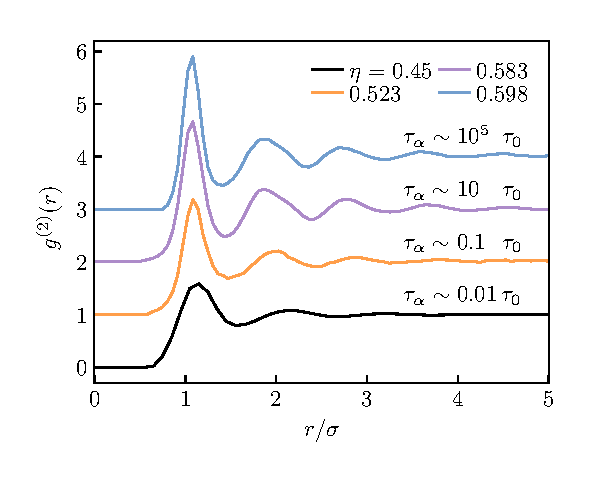
\includegraphics[width=0.9\linewidth,outer]{g2-evolution}
  %\missingfigure[figwidth=\linewidth]{$g^{(2)}$}%
  \caption[Structural change in the supercooled liquid (at the pair level)]{
    Minimal change occurring in pairwise structure of hard spheres as density is increased above the melting point, as measured by the pair distribution function \eqref{eq:n-particle-distribution}.
    Each state-point is offset for clarity.
    Results for $\eta = 0.45$ for a 7-component equimolar mixture with 16\% polydispersity using the DynamO software package \cite{BannermanJCC2011}, whereas the data in the metastable regime is from colloidal experiments provided by the authors of Ref.\ \cite{HallettNC2018}.
  }
  \label{fig:g2-changes}
\end{SCfigure}

Structurally, supercooled liquids are not meaningfully different from their ordinary counterparts.
Operationally, a supercooled liqiud is equilibrated in the sense that all observables are time independent and the thermodynamics is self-consistent%
\marginfootnote{Different routes to measuring thermodynamic quantities, e.g.\ the pressure, may give different values in an out-of-equilibrium system.
  This is not the case in supercooled liquids, even though they are not strictly in equilibrium.}.
Formally speaking, the system is sometimes said to be in \emph{local equilibrium}, where it samples all the liquid microstates ergodically; or that it obeys \emph{detailed balance}, where the dynamics is microscopically reversible.
%have very similar structural characteristics as at equilibrium.
As a consequence, the liquid loses any memory of its preparation and all observables become time independent.
That is, for some observable $A$ we can write
\begin{equation*}
  \langle A(t) \rangle = \langle A \rangle.
\end{equation*}
This includes the static correlation functions, introduced in section \ref{sec:liquid-structure}, which remain well-defined in the supercooled regime.
Furthermore, the pair distribution function $g^{(2)}(r)$ is seen to change very little as the density (or temperature) is increased (decreased) from the normal liquid; as an example, we show this for hard spheres in Fig.\ \ref{fig:g2-changes}.
As pair correlations are the main measure of structure in simple liquids, this suggests minimal structural change occurs in the high density liquid.
As a corollary, time correlation functions become \emph{time-translation invariant} meaning they depend only on time differences i.e.\
\begin{equation*}
  \langle A(t) A(t') \rangle = \langle A(0) A(t - t') \rangle.
\end{equation*}

A more sophisticated way in which supercooled liquids can be thought of as equilibrium systems involves the response functions.
In an equilibrium system, the response of a system to a small perturbation is directly related to the microscopic source of fluctuations%
\marginfootnote{Temperature, in the case of liquids.}.
The \emph{fluctuation-dissipation relation} for an observable $A$ expresses the system's susceptibility to perturbation as
\todo{Check this equation is correct against a textbook, get a citation.}
\begin{equation*}
  \chi_A (t, t')
  =
  - \beta \Theta(t - t')
  \frac{d}{dt}
  \left(
  \bigg\langle
  (A(t - t') - \langle A \rangle)
  (A(0) - \langle A \rangle)
  \bigg\rangle
  \right)
\end{equation*}
where the Heaviside theta function imposes causality.
These relations are obeyed in supercooled liquids, even though they are not a proper equilibrium state.

Now we turn to discussing the ways in which supercooled liquids are markedly different from normal liquids: in their \emph{dynamics}.
Typically this is discussed in the context of two (related) quantities: the \emph{viscosity} and the \emph{relaxation time}.
Viscosity measures how resistant the system is to flow, while relaxation time measures the typical microscopic time for the density profile to relax i.e.\ for liquid-like behaviour caused by particle diffusion.
A defining feature of supercooled liquids is that these numbers become so large that the precise details of the measurement used does not matter.
We will discuss this dynamical slowdown further on, but for now we introduce a specific time correlation function in order to frame the discussion.
A popular measurement is the intermediate scattering function (ISF), defined by \cite{JanssenFP2018}
\begin{equation}\label{eq:isf}
  F(k, t)
  =
  \frac{
    \big\langle \tilde{\rho}(\vec{k}, t) \tilde{\rho}(-\vec{k}, 0) \big\rangle
  }{
    \langle N \rangle
  }
\end{equation}
which reduces to the static structure factor \eqref{eq:static-structure-factor} at zero elapsed time $F(k, t=0) = S^{(2)}(k)$.
An example ISF is shown in Fig.\ \ref{fig:isf}, displaying many features which distinguish the supercooled liquid from a regular liquid.
In particular, there is a timescale separation between distinct dynamical processes.
For short times there is a ballistic regime, where particles are essentially free to move unencumbered.
At intermediate times, interactions with neighbours inhibit motion and $F(k,t)$ plateaus; this plateau is absent in regular liquids.
Finally, in the long time limit particles are able to diffuse so that $F(k,t)$ completely relaxes to zero.
The latter two processes are called $\beta$- and $\alpha$-relaxation respectively.
The timescale of the longer $\alpha$-relaxation $\tau_\alpha$ is more central to our discusson as it corresponds to the timescale of liquid-like behaviour.

\begin{SCfigure}
  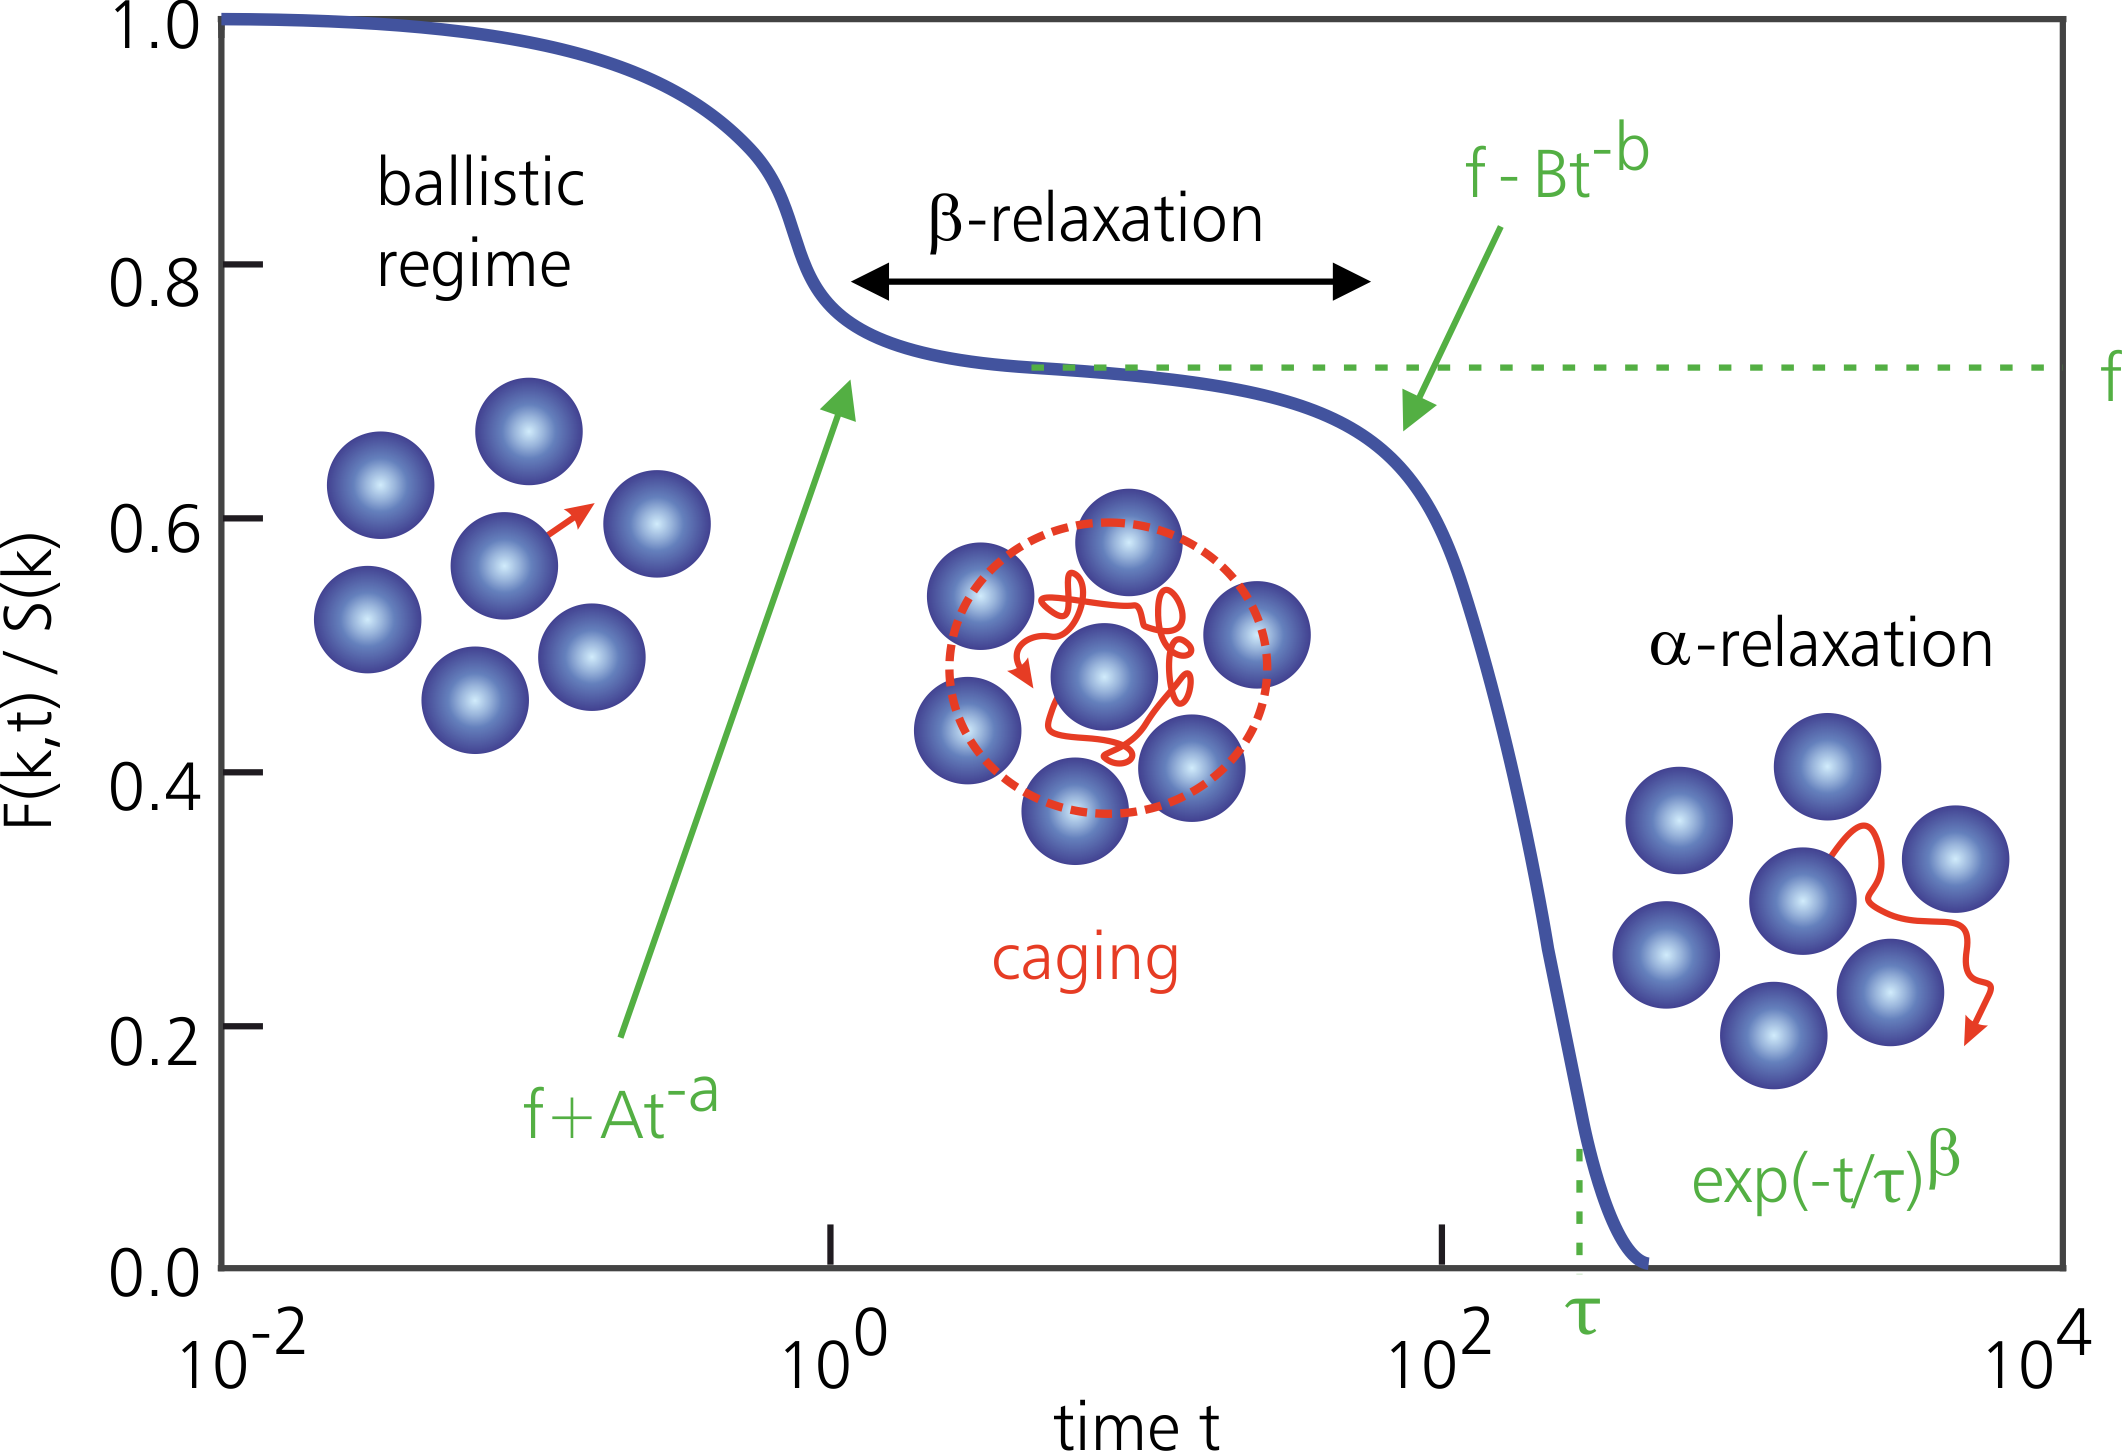
\includegraphics[width=0.9\linewidth,outer]{isf}
  \caption[Intermediate scattering function in a supercooled liquid]{
    Typical intermediate scattering function in a supercooled liquid.
    The power law predictions are from mode-coupling theory.
    Reproduced from Ref.\ \cite{JanssenFP2018}.
  }
  \label{fig:isf}
\end{SCfigure}

A helpful framework to guide discussion of dynamical processes is \emph{transition state theory}.
In this approach a dynamical process, e.g.\ a chemical reaction, is imagined to occur through a dynamical bottleneck (Fig.\ \ref{fig:transition-state}).
We imagine evaluating a thermodynamic potential%
\marginfootnote{Which thermodynamic potential this corresponds to will depend on the ensemble.}
$\Phi$ at every point along the reaction path.
The process will then be limited by the rate of thermal fluctuations of size $\Delta \Phi$, i.e.\ those able to reach the transition state.
In equilibrium, the timescale for the process will then scale by the Boltzmann weight
\begin{equation}\label{eq:reaction-time}
  \tau \sim e^{\beta \Delta \Phi}.
\end{equation}
There will be additional kinetic prefactors out in front, however for large barriers we expect the thermodynamic contribution to dominate because of its exponential weighting.
This framework can be more rigorously justified through e.g.\ an \emph{instanton} approach \cite{LangerAP1969}.
The main limitation of transition state theory is the assumption that dynamical processes occur through effectively one-dimensional reaction paths; later, we will introduce a more sophisticated form of this framework which considers the high dimensional \emph{energy landscape}.

As an example of how useful transition state theory can be, we very briefly consider \emph{classical nucleation theory} which we will return to in more detail in chapter \ref{chapter:aerosols}.
Imagining crystallisation to occur by the spontaneous formation of the new phase inside of the liquid, then the timescale for this process will scale as
\begin{equation*}
  \tau_\mathrm{crys} \sim e^{ \beta \Delta \Phi_\mathrm{crys}}.
\end{equation*}
Then, assuming a temperature-independent barrier $\Delta \Phi_\mathrm{crys}$, the timescale for nucleation will increase exponentially as temperature is lowered allowing for the supercooled liquid to become long-lived \cite{CavagnaPR2009}.
%This is essentially the reason it is possible for supercooled liquids to exist at all, and reach an effectively time-translation invariant state without decaying to the crystal \cite{CavagnaPR2009}.
This argument is highly system dependent, as systems with small barriers to crystallisation will not be long-lived enough for a metastable supercooled phase to be observed.
Single-component hard spheres are particularly prone to crystallise at very high densities, so polydispersity is typically introduced to frustrate the crystal structure and extend the lifetime of the supercooled liquid.
This is an imperfect process however, as even highly polydisperse systems have been found to crystallise \cite{BommineniPRL2019,BerthierPRL2016}.

\begin{SCfigure}
  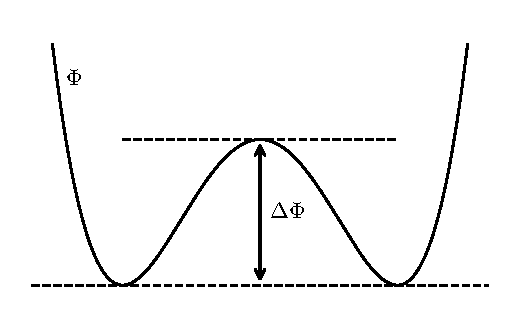
\includegraphics[width=0.7\linewidth,center]{transition-state}
  \caption[Transition state theory]{
    A double-well potential featuring a barrier $\Delta\Phi$, representing the minimum energy required for the system to pass between the two \emph{basins}.
    The $x$-axis is the \emph{reaction coordinate}, representing a one-dimensional projection of the complete degrees of freedom.
  }
  \label{fig:transition-state}
\end{SCfigure}

Applying transition-state theory \eqref{eq:reaction-time} to relaxation time in the liquid, we may expect the $\alpha$-relaxation time to scale as
\begin{equation}\label{eq:tau-barrier}
  \tau_\alpha \sim e^{\beta \Delta \Phi_\alpha}
\end{equation}
where $\Delta \Phi_\alpha$ is the barrier to relaxation.
Naively, we might expect the barrier to remain constant with temperature, corresponding to e.g.\ the cost of breaking a chemical bond, then we arrive at the Arrhenius law
\begin{equation}\label{eq:arrhenius-law}
  \ln{\tau_\alpha} \propto \frac{1}{T}.
\end{equation}
This argument captures the high temperature behaviour very well and, outside of soft matter, it applies reasonably well to many molecular glassformers e.g.\ silica-based materials%
\marginfootnote{That is, the material which the average person would mean when they say ``glass''.},
where relaxation essentially depends on the timescale to break a covalent bond.
Experimental data for \ce{SiO2} \cite{AngellS1995} confirms that $\ln{\tau_\alpha}$ scales linearly with $\beta$ (Fig.\ \ref{fig:angell}).
By convention, systems which scale in an Arrhenius fashion are called \emph{strong}%
\marginfootnote{This baffling naming convention has nothing to do with the mechanical properties.}
glassformers.

Our focus is on soft matter, with hard spheres as the prototypical model, where the  chemical bonds (typically van der Waals attractions) are much weaker than in molecular systems (and absent in hard spherse).
Consequently, there is less of a case for an Arrhenius relationship \eqref{eq:arrhenius-law}, and empirically we find striking deviations from it.
Many systems show \emph{super-Arrhenius} scaling with temperature (Fig.\ \ref{fig:angell}), including mixtures of Lennard-Jones atoms and molecular orthoterphenyl.
Correspondingly, systems where $\tau_\alpha$ scales faster than exponential are labelled as \emph{fragile}.

Some modification is required for hard particle systems, where temperature is not a natural control parameter.
As we argued in the introduction, pressure is the only meaningful state variable.
The authors of Ref.\ \cite{BerthierPRE2009} argue that pressure plays a role equivalent to inverse temperature in athermal systems, because of similarities in their limit behaviour.
Alternatively, we could make a free volume argument, where we expect a relaxation event to involve fluctuations of volume $\Delta V$.
In equilibrium, volume fluctuations are created by reversible work $p \Delta V$ so to leading order%
\marginfootnote{The leading order behaviour can be given more justification by invoking the morphometric approach \eqref{eq:fmt-morphometric-2}, or from more general arguments which we will introduce in section \ref{sec:insertion-as-solvation}.}
we then expect
\begin{equation*}
  \tau_\alpha \sim e^{\beta p \Delta V}.
\end{equation*}
Taking $\Delta V$ as the equivalent of an energy barrier, we find the conjugate variable $\beta p$ does indeed play the role of inverse temperature.
It is usual to work with the dimensionless \emph{compressibility factor}, defined by
\begin{equation}
  Z = \frac{\beta p}{\rho},
\end{equation}
in terms of which hard spheres show the same phenomenology as thermal systems in Fig.\ \ref{fig:angell}.
We find hard spheres are comparable in fragility to various binary Lennard-Jones mixtures.

\hl{Things I have not yet mentioned:}
\begin{itemize}
\item \hl{glass transition: 100s}
\item \hl{operationally, what it looks like in thermodynamic potentials as the system falls out of equilibrium.}
\item \hl{dynamical heterogeneities (can probably save this until mentioning facilitation though)}
\item \hl{Stokes-Einstein breakdown}
\end{itemize}

%% We discussed the static correlation functions at length, which is fine for liquids where equilibrium occurs on a \SI{100}{\pico\second} timescale.
%% Dynamical effects are highly nontrivial at high densities.
%% As a practical definition, a glass is defined in the lab as any material for which the relaxation time exceeds \SI{100}{\second}: this point is called the experimental glass transition.
%% This is somewhat arbitrary, although the location of the glass transition point is not particularly sensitive to where you set the threshold because of how rapidly the viscosity/times are increasing around there.
%% So what do we mean by dynamical arrest.

%% Cooling a liquid.
%% Take thermodynamic quantity (e.g.\ volume, entropy, enthalpy): usually crystallise.
%% (Picture)
%% First-order transition bypassed by quick cooling.
%% Enter supercooled liquid phase.

%% Both of these conditions are violated in the glass, as this is a truly non-equilibrium state.
%% That is, we see ageing, and hysteresis in response to perturbations.
%% No longer equilibrates/relax/flows, call it a glass: occurs at glass transition.
%% Glass is a solid for all practical purposes.
%% Distinguished from glass which has dependence on preparation history, hysteresis/memory effect of heating the system (will not follow exactly the same curve until - back to the equilibrium supercooled structure), aging: averages (including correlations) evolve in time.

%% The glass transition itself is not a ``transition'' in the thermodynamic sense; there is no.
%% It's really a kind of impatience transition; the glass transition for a human would be different to the glass transition for a demigod/ent.
%% It's still a relatively robust measurement, because of the superarrhenius scaling (sc-l for pedestrians).

%% A plethora of questions related to the out-of-equilibrium properties.
%% \begin{enumerate}
%% \item Properties of out of equilibrium glass phase: very important questions for material science. Low temperature anomalies, aging behaviour, nonlinear rheology  plasticity.
%% \item Relation between glass and jamming. Jamming=zero temperature, out of equilibrium, infinite pressure.
%% \item How to avoid crystallisation.
%% \end{enumerate}

A super-Arrhenius scaling of $\tau_\alpha$ implies that the thermodynamic barrier itself $\Delta \Phi_\alpha$ increases with supercooling.
This means that the dynamics fundamentally changes at high densities (or low temperatures), which must be caused by the onset of \emph{collective} effects%
\marginfootnote{Also referred to as \emph{cooperative} effects.};
given the weakness of bonds in soft matter, we can conclude that many particles must contribute to create a large barrier.
We will discuss this more in the next section.
Relaxation barriers in hard spheres are entropic in nature, so perhaps it is easier to see the need for collective effects.
Moreover, the geometrical interpretation in terms of volume fluctuations $\Delta V$ provides a picture for collective motion: at high densities more particles will have to move out of the way to create the space for motion.

\begin{SCfigure}
  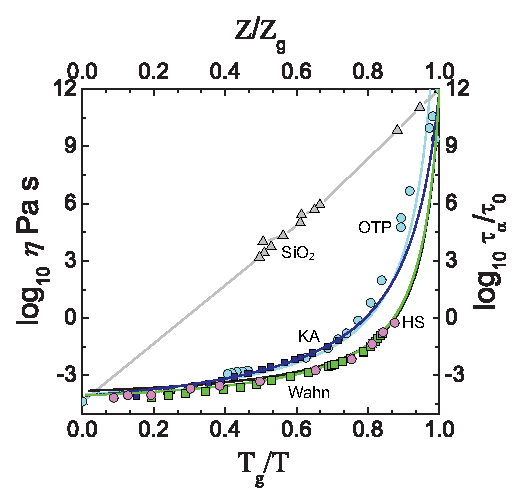
\includegraphics[width=0.9\linewidth,outer]{angell}
  \caption[Angell plot]{
    The \emph{Angell} plot \cite{AngellJNS1988} for molecular and model glassformers showing the temperature/pressure dependence of viscosity $\eta$ (or equivalently relaxation time $\tau_\alpha$).
    The molecular systems \ce{SiO2} and orthoterphenyl (OTP) respectively display the \emph{strong} and \emph{fragile} behaviours described in text, with data obtained from Refs.\ \cite{AngellS1995, BerthierPRE2009}.
    Kob-Anderson (KA) and Wahnstrom (Wahn) are binary mixtures of Lennard-Jones atoms designed to exhibit fragility.
    The compressibility $Z = \beta p / \rho$ is argued to be equivalent to inverse temperature for hard spheres (HS) \cite{BerthierPRE2009}, with data taken from Ref.\ \cite{RoyallJSM2017}.
    Reproduced from Ref.\ \cite{RoyallPR2015}.
  }
  \label{fig:angell}
\end{SCfigure}

%% We will talk about this metastable branch as if it were in equilibrium.
%% \todo{create link when mention high density swap data}

%% Relationship with viscosity.
%% Flowing/not flowing is captured by viscosity: viscous slowdown same as relaxation slowdown.
%% Slightly different notion.
%% Short times $t \ll \tau$: elastic system, long times $t \gg \tau$: viscosity.
%% Time barrier is relaxation time.
%% Elasticity, viscosity in Newtonian fluids: viscoelastic behaviour (Maxwell)
%% \begin{equation}
%%   \eta = G_\infty \tau_\mathrm{relax}
%% \end{equation}
%% high frequency shear modulus is elastic property.
%% Shear modulus increases by factor 2-5 times, is dwarfed by change in relaxation time.

\subsection{Mode-coupling theory}

Reviews: \cite{ReichmanJSM2005, JanssenFP2018}

We start with an explicitly dynamical theory.
Central idea: \emph{slow} and \emph{fast} variables.

To motivate mode-coupling theory we start from the classical Langevin equation of motion, which expresses the equations of motion of a subset of the degrees of freedom.
Newton's equation becomes
\begin{equation*}
  m \ddot{\vec{r}} = - \lambda \dot{\vec{r}} + \vec{F}(t)
\end{equation*}
where $\vec{F}$ is a Gaussian random field
\begin{equation*}
  \langle F_i(t) F_j(t') \rangle = 2 D \delta_{i,j} \delta(t - t').
\end{equation*}
This equation is valid where there is a timescale separation between \emph{slow} and \emph{fast} variables: the position $\vec{r}$ represents a slowly evolving variable of interest, whereas the remaining degrees of freedom (e.g.\ small solvent particles) are imagined to equilibrate rapidly leaving only the force field $\vec{F}$.

In mode-coupling theory, an \emph{exact} generalised Langevin equation is derived as
\begin{equation}
  \frac{d \vec{x}(t)}{dt}
  =
  i \vec{\Omega} \cdot \vec{x}
  - \int_0^t \vec{K} \cdot \vec{x}(t - t') \, dt'
  + \vec{f}(t)
\end{equation}
where $\vec{\Omega}$ is frequency matrix, $\vec{K}$ is a time-dependent \emph{memory function}, and $\vec{f}$ is the fast fluctuating force.

The full MCT equation
\begin{equation}
  \frac{d^2 F(k,t)}{d t^2}
  + \frac{k^2}{\beta m S(k)} F(k, t)
  + \int_0^t K_\mathrm{MCT}(k, t') \frac{d F(k, t - t')}{dt} \, dt'
  =
  0
\end{equation}
with the memory function given by
\begin{equation}
  K_\mathrm{MCT}
  =
  \frac{\rho}{16 \pi^3 \beta m}
  \int |V_{\vec{q},\vec{k}-\vec{q}}|^2
  F(q, t) F(|\vec{k} - \vec{q}|, t)
  \, d\vec{q}.
\end{equation}

Predicts a diverging timescale.
Nevertheless, liquids can be prepared above this volume fraction in colloidal experiments \cite{BrambillaPRL2009} and simulations \cite{BerthierPRL2016}.

The point of this section is to indicate that pair correlation functions are not enough.
Extensions with higher order structure \cite{JanssenPRL2015,JanssenFP2018}.

\subsection{Mean-field theory}

A growing consensus is forming around this explanation.
Inspired by the solutions of mean-field spin glasses, the great breakthrough of the original papers was that these systems were identical in the structure of the energy landscape.
Connection between thermodynamics and dynamics, configurational entropy.
This argument is thermodynamic, which in some sense is structural.
Structural in the sense of the energy landscape, not necessarily in real space/local structure.
Compatible with MCT, in fact high dimensional calculations lead to a theory almost identical to MCT \cite{MaimbourgPRL2016,KurchanJSM2016}.

The relevance of mean-field theory in physical dimensions comes from an interpretation \cite{KirkpatrickPRB1987, KirkpatrickPRA1989}, and antecedent ideas found in \cite{AdamJCP1965}.
RFOT: argument of Ref.\ \cite{BouchaudJCP2004}, introduces point-to-set length.

Point-to-set length is the minimum size of a subsystem for there to be relaxation: the space of states transitions from being a single state (point) to a multitude of states (set).
It can be rigorously proven that a diverging timescale necessarily must coincide with a diverging point-to-set length: Montanari \cite{MontanariJSP2006}.
The essence of the argument is that for a finite subsystem, there will be a finite barrier, so any dynamics must scale Arrheniusly.
Therefore, the relaxation time will be bounded from above by the dynamical lengthscale, and super-Arrhenius scaling suggests growing collective behaviour.

This must trivially occur at the very least $T=0\si{K}$ where relaxation timescales diverges, however much like the lack of a phase transition in the Ising model in $d=1$ this is not a true thermodynamic phase transition because it cannot be crossed.
Recent numerical evidence suggests that a model glassformer in $d=2$ does not show a transition, also vanishing at $T=0\si{K}$ \cite{BerthierNC2019}.
So the central question of glass is what happens in $d=3$, is there a vanishing configurational entropy at a finite $T > 0$ with an accompanying thermodynamic glass transition?
In mean-field, formally in the limit of infinite spatial dimensions $d \to \infty$, the hard sphere system has been shown to have a true transition, however the critical dimensions are unknown so it is unclear what happens in $d=3$. \cite{KurchanJSM2012,KurchanJPCB2013,CharbonneauNC2014,CharbonneauJSM2014}.

\begin{SCfigure}
  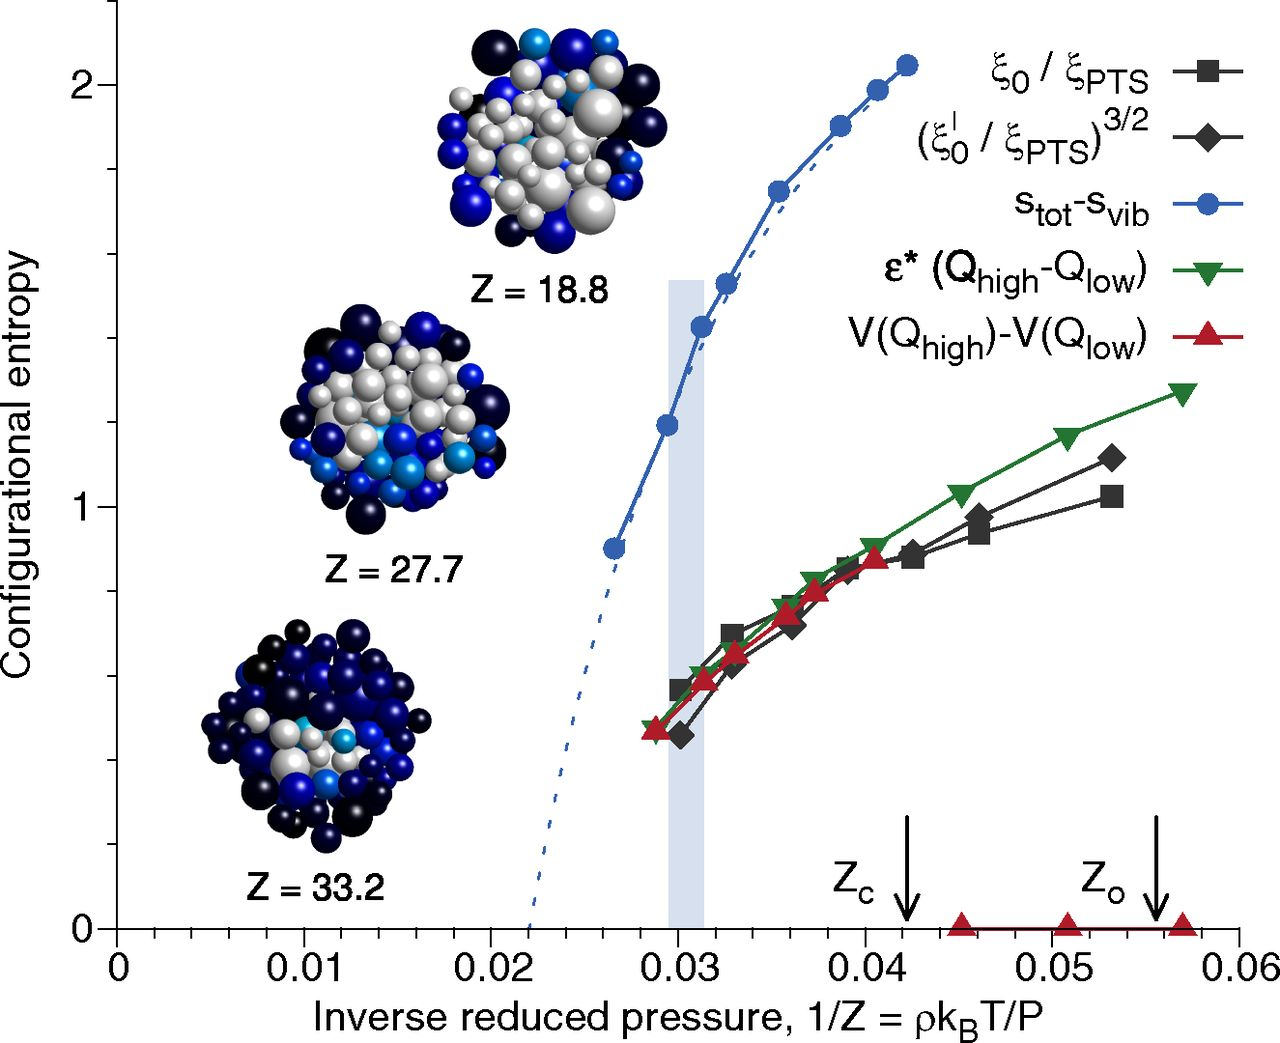
\includegraphics[width=0.9\linewidth,outer]{swap-Sconf}
  \caption[Configurational entropy in hard spheres from Monte-Carlo simulations]{
    Configurational entropy in hard spheres from novel Monte-Carlo (MC) simulations for a system with 23\% polydispersity.
    The various methods used (described in Ref.\ \cite{BerthierPNAS2017}) all broadly agree that this quantity is trending to zero at a finite pressure, suggesting the existence of a thermodynamic glass transition.
    The equation of state for this system is given in Fig.\ \ref{fig:swap-eos}.
    Reproduced from Ref.\ \cite{BerthierPNAS2017}.
  }
\end{SCfigure}

\subsection{Local structure picture}

Stripmine Paddy's review for this section \cite{RoyallPR2015}.

In conventional condensed matter physics dynamics is determined by structure.
For example, crystalline solids are fixed on a lattice so do not flow, whereas liquids are disordered and are thus able to flow.
Soft matter systems (e.g.\ gels, foams, glasses) do not neatly fall into this paradigm: their dynamics are often arrested whilst their structure remains highly disordered.

Frustration-limited domain theory \cite{TarjusJPCM2005}.

Previous viewpoints, MCT and mean-field, are structural in the sense of being thermodynamic; however they do not explicitly invoke local structure.
That being said, they are broadly compatible viewpoints.
After all, emergence of a structural motif would be sufficient to reduce the configurational entropy (or a manifestation of this, depend on one's viewpoint).

Glotzer picture: competition between competing structures \cite{TeichNC2019}.

\subsection{Other viewpoints: jamming and facilitation}

Theories concentrating on the high density glass: elastic theories.
Dynamic facilitation.

\subsection{Perspective: role of many-body correlations}

To motivate the use of many-body correlations we employ an argument due to Evans \cite{EvansPrivate2019}.
In section \ref{sec:thermodynamic-routes} we saw how the compressibility and virial routes lead to expressions of the free energy in terms of pair correlations.
This is emblematic of conventional routes to the free energy, so in some sense all of the thermodynamically relevant information is contained in the two body correlation functions.
However, the pair correlation yields thermodynamic quantities which are \emph{derivatives} of the free energy at an instantaneous state point, so to infer the free energy we must sample multiple state points.
Equivalently, we could consider the derivatives of the pair correlation function.
It is straightforward to show that \cite{Santos2016}
\begin{equation}\label{eq:correlation-derivatives}
  \chi_T \rho
  \left( \frac{\partial \rho^{(n)}}{\partial \rho} \right)_{V,T}
  =
  (n - \rho V) \rho^{(n)}(\vec{r}^n)
  + \int \rho^{(n+1)}(\vec{r}^{n+1}) \, d\vec{r}_{n+1}.
\end{equation}
The important feature to take away from this expression is the presence of $\rho^{(n+1)}$; we see that higher-order correlations emerge in the derivatives.
This means we could in principle measure the free energy at a single state point by introducing highly accurate measurements of the many-body correlation functions.
This is essentially the spirit of the \emph{entropy route}, which writes \cite{WallaceJCP1987}
\begin{equation}
  S = \sum_{n=1}^\infty S_n
\end{equation}
with entropic terms $S_n$ containing contributions from $n$-particle correlations.
The first few terms are given by \cite{WallaceJCP1987}
\begin{subequations}
  \begin{align}
    \frac{S_1}{V}%\langle N \rangle}
    &=
    k_B \, \rho \left( \frac{d}{2} - \ln{\rho \Lambda^d} \right),
    \\
    \frac{S_2}{V}%\langle N \rangle}
    &=
    \frac{\rho^2}{2 T}
    \int g^{(2)}(\vec{r}) \ln{g^{(2)}(\vec{r})}
    \, d\vec{r},
    \\
    \frac{S_3}{V}%\langle N \rangle}
    &=
    \frac{\rho^3}{6 T}
    %\int g^{(3)}(\vec{r}, \vec{r}') \delta w^{(3)}(\vec{r}, \vec{r}')
    \int g^{(3)}(\vec{r}, \vec{r}')
    \ln{\left(
      \frac{
        g^{(3)}(\vec{r}, \vec{r}')
      }{
        g^{(2)}(\vec{r}) g^{(2)}(\vec{r}') g^{(2)}(\vec{r} - \vec{r}')
      }
      \right)}
    \, d\vec{r} d\vec{r}'.
  \end{align}
\end{subequations}

Second, while it is true that thermodynamic quantities like the pressure can certainly be inferred from the pair correlations, there is no such simple relationship for dynamic quantities.
In the absence of a thermodynamic phase transition, we would not expect the pair correlation to reveal much about the nature of dynamical arrest, beyond the lack of a transition.
And even supposing the existence of a transition, the precision required to detect such a signal $g(r)$ may be arbitrarily subtle; however, any the changes approaching a transition \emph{must} be magnified in the higher order correlation functions because of \eqref{eq:correlation-derivatives}.
This is particularly true as we saw \hl{local mechanisms in the various theories}.

We will be focusing on many-body correlations in real space, to explore the local mechanisms proposed in theories of the glass transition mentioned above.
In some situations the correlations in Fourier space may be more useful, most notably in MCT where many-body generalisations have already found some traction \cite{JanssenPRL2015,JanssenFP2018}.
In principle, our real space correlation functions can be Fourier transformed to obtain these functions, but in practice this is prohibited by the high dimensionality of the correlation functions for even modest $n$.
However, we indicate below how FMT already provides an easy route to obtaining all the correlation functions in Fourier space, as described by the original papers \cite{RosenfeldPRL1989,RosenfeldJCP1990}.

Fourier transforming the direct correlation functions for the uniform liquid \eqref{eq:fmt-direct-correlations-uniform-density}, and applying the convolution theorem, allows us to write the rather succinct
\begin{equation}
  \tilde{c}^{(n)}(\vec{k}^n)
  =
  - \sum_{\alpha_1, \alpha_2, \cdots, \alpha_n}
  \partial^n_{\alpha_1, \alpha_2, \cdots, \alpha_n} \beta f^\mathrm{ex} \;
  \left( \prod_{i=1}^n \widetilde{\omega}_{\alpha_i}(\vec{k}_i) \right)
  \delta(\vec{k}_1 + \vec{k}_2 + \cdots + \vec{k}_n).
\end{equation}
The delta function enforces the `ring' condition $\sum_{i=1}^n \vec{k}_i = 0$ which emerges from translational symmetry of the weight functions, reducing the dimensionality of the domain by $d$.
A further $d(d-1)/2$ degrees of freedom%
\marginfootnote{This many degrees of freedom can be removed for general $n \ge d$, but we expect fewer for $n < d$.
  For example, $n=2$ arrangements (a dimer) are isomorphic to a line so they possess $d-1$ rotational degrees of freedom.}
can be removed by exploiting rotational symmetry.
Many-particle generalisations of the static structure factor can be obtained from $\tilde{c}^{(n)}(\vec{k}^n)$ by functionally differentiating the Ornstein-Zernike equation \eqref{eq:ornstein-zernike-generic} with respect to density \cite{BarratMP1988}.

This concludes the relevant background on liquid state theory.
In subsequent chapters we will develop a framework for treating the many-body correlation functions in real space.
